\documentclass[letterpaper,superscriptaddress,showkeys,longbibliography,10pt]{revtex4-1}\usepackage{graphicx, color}
%% maxwidth is the original width if it is less than linewidth
%% otherwise use linewidth (to make sure the graphics do not exceed the margin)
\makeatletter
\def\maxwidth{ %
  \ifdim\Gin@nat@width>\linewidth
    \linewidth
  \else
    \Gin@nat@width
  \fi
}
\makeatother

\IfFileExists{upquote.sty}{\usepackage{upquote}}{}
\definecolor{fgcolor}{rgb}{0.2, 0.2, 0.2}
\newcommand{\hlnumber}[1]{\textcolor[rgb]{0,0,0}{#1}}%
\newcommand{\hlfunctioncall}[1]{\textcolor[rgb]{0.501960784313725,0,0.329411764705882}{\textbf{#1}}}%
\newcommand{\hlstring}[1]{\textcolor[rgb]{0.6,0.6,1}{#1}}%
\newcommand{\hlkeyword}[1]{\textcolor[rgb]{0,0,0}{\textbf{#1}}}%
\newcommand{\hlargument}[1]{\textcolor[rgb]{0.690196078431373,0.250980392156863,0.0196078431372549}{#1}}%
\newcommand{\hlcomment}[1]{\textcolor[rgb]{0.180392156862745,0.6,0.341176470588235}{#1}}%
\newcommand{\hlroxygencomment}[1]{\textcolor[rgb]{0.43921568627451,0.47843137254902,0.701960784313725}{#1}}%
\newcommand{\hlformalargs}[1]{\textcolor[rgb]{0.690196078431373,0.250980392156863,0.0196078431372549}{#1}}%
\newcommand{\hleqformalargs}[1]{\textcolor[rgb]{0.690196078431373,0.250980392156863,0.0196078431372549}{#1}}%
\newcommand{\hlassignement}[1]{\textcolor[rgb]{0,0,0}{\textbf{#1}}}%
\newcommand{\hlpackage}[1]{\textcolor[rgb]{0.588235294117647,0.709803921568627,0.145098039215686}{#1}}%
\newcommand{\hlslot}[1]{\textit{#1}}%
\newcommand{\hlsymbol}[1]{\textcolor[rgb]{0,0,0}{#1}}%
\newcommand{\hlprompt}[1]{\textcolor[rgb]{0.2,0.2,0.2}{#1}}%

\usepackage{framed}
\makeatletter
\newenvironment{kframe}{%
 \def\at@end@of@kframe{}%
 \ifinner\ifhmode%
  \def\at@end@of@kframe{\end{minipage}}%
  \begin{minipage}{\columnwidth}%
 \fi\fi%
 \def\FrameCommand##1{\hskip\@totalleftmargin \hskip-\fboxsep
 \colorbox{shadecolor}{##1}\hskip-\fboxsep
     % There is no \\@totalrightmargin, so:
     \hskip-\linewidth \hskip-\@totalleftmargin \hskip\columnwidth}%
 \MakeFramed {\advance\hsize-\width
   \@totalleftmargin\z@ \linewidth\hsize
   \@setminipage}}%
 {\par\unskip\endMakeFramed%
 \at@end@of@kframe}
\makeatother

\definecolor{shadecolor}{rgb}{.97, .97, .97}
\definecolor{messagecolor}{rgb}{0, 0, 0}
\definecolor{warningcolor}{rgb}{1, 0, 1}
\definecolor{errorcolor}{rgb}{1, 0, 0}
\newenvironment{knitrout}{}{} % an empty environment to be redefined in TeX

\usepackage{alltt}

\usepackage[utf8]{inputenc}
\usepackage{color,dcolumn,graphicx,hyperref}
\usepackage{natbib}
\usepackage{footnote}
\hypersetup
{
  colorlinks = true, linkcolor = blue, citecolor = blue, urlcolor = blue,
}

\begin{document}




\title{taxize - taxonomic search and retrieval in R}

\author{Scott Chamberlain}
\email[E-mail: ]{myrmecocystus@gmail.com}
\affiliation{Biology Department, Simon Fraser University, Canada.}

\author{Eduard Sz\"{o}cs}
\email[E-mail: ]{szoe8822@uni-landau.de}
\affiliation{Institute for Environmental Sciences, University Koblenz-Landau, Forststraße 7, 76829 Landau, Germany}
\keywords{taxonomy; R; software; data; API}

\maketitle

\section{Abstract}

All species are hierarchically related to one another, and we use taxonomic names to label the nodes in this hierarchy. Taxonomic data is becoming easily available on the web, but scientists need a way to access taxonomic data on the web in a programmatic fashion, which is fast and reproducible. We have developed taxize, an open-source software package (freely available from \url{http://cran.r-project.org/web/packages/taxize/index.html}) for the R language. taxize provides a simple, programmatic access to taxonomic data for 13 data sources around the web. We discuss the need for a taxonomic toolbelt in R, and outline a suite of use cases for which taxize is ideally suited (including a full workflow as an appendix). The taxize package will facilitate open and reproducible science by allowing taxonomic data collection to be done in the open-source R platform.

\section{Introduction}

Evolution by natural selection has led to a hierarchical relationship among all living organisms.  Thus, species are categorized using a taxonomic hierarchy, starting with the binomial species name (e.g, \emph{Homo sapiens}), moving up to genus (\emph{Homo}), then family (\emph{Hominidae}), and on up to Domain (\emph{Eukarya}). Biologists, whether studying organisms at the cell, organismal, or community level, can put their study taxa into taxonomic context, allowing them to know close and distant relatives, find relevant literature, and more. Discovering the correct taxonomic names is, unfortunately, not straightforward. Taxonomic names often change due to name changes at the generic or specific levels, lumping or splitting lower taxa (genera, species) among higher taxa (families), and name spelling changes. In addition, there is no one authoritative taxonomic names source. Instead, there are essentially competing sources (e.g., uBio, Tropicos, ITIS) that may have different accepted names for the same taxon. The goal of taxize, an R package in development, is to make all use cases having to do with taxonomy easy and replicable. 

Taxonomic data is getting easier to obtain through web interfaces (e.g., \url{http://eol.org/}). However, there are a number of good reasons to obtain taxonomic information programatically rather than through a web interface. First, if you have more than a few names to lookup on a website, it can take quite a long time to enter each name, get data, and repeat for each species. Second, programatically getting taxonomic names solves the first problem by looping over a list of names, and is reproducible. With increasing reports of irreproducibility in science \cite{stodden2010,zimmer2012}, it is extremely important to make science workflows repeatable. 

The R language is the dominant language used by biologists (reference), and now has over 4,000 packages on the main repository (CRAN) and more than 2,500 packages on other repositories to extend R. R is great for manipulating, visualizing and fitting statistical models to data. However, the key missing piece in R is the ability to get data within R. Increasingly, data is available from the web via API's, or application programming interfaces. These are bits of code that allow computers to talk to one another. Web APIs define a number of methods that allow users to search for a species name, or retrieve the synonyms for a species name, for example. One can then write functions in any programming language to interact with the API, allowing users to interact with the web API without having to know the details of the code. In taxize, we have written a suite of R functions that interact with many taxonomic data sources via their web APIs (Table~\ref{tab:a}). The interface to each function is usually a simple list of species names, just as user would do with a web API.

\section{Why taxize?}

There are a large suite of applications developed around the problem of searching for, resolving, and getting higher taxonomy for species names. For example, Linnaeus \url{http://linnaeus.sourceforge.net/} provides ability to search for taxonomic names in documents and normalize names. In addition, there are many web interfaces to search for and normalize names such as Encyclopedia of Life's Global Names Resolver \url{http://resolver.globalnames.org/}, uBio tools \url{http://www.ubio.org/index.php?pagename=sample_tools}, and iPlant's Taxonomic Name Resolution Service \url{http://tnrs.iplantcollaborative.org/}. 

All of these tools provide great ways to search for taxonomic names and resolve them in some cases. However, scientists ideally need a tool that can be used programmatically, and thus be made reproducible, and highly customizeable. The goal of taxize is to make it easy to create reproducible and easy to use workflows for searching for taxonomic names, resolving them, getting higher taxonomic names, and other tasks related to research dealing with species. 

\section{Data sources}

taxize uses many data sources (Table~\ref{tab:a}), and more can easily be added. There are two common tasks provided by the data sources: name search and name resolution. Other functionality in taxize includes retrieving a classification tree for a species, or retrieving child taxa of a focal taxon. One of the data sources (Phylomat) returns phylogenies, while another (NCBI) returns genetic sequence data. However, there are other R packages that are focused solely on sequence data, such as rsnps \cite{chamberlain2013}, rentrez \cite{winter2013}, BoSSA \cite{lefeuvre2010}, and ape \cite{paradis2004}. 

Some of the data sources taxize interacts with require authentication. That is, in addition to the search terms you provide (e.g., \emph{Homo sapiens}), they require an alphanumeric identification key so that they can better manage their data. The services that do require an API key are: Encyclopedia of Life (EOL), the Universal Biological Indexer and Organizer (uBio), Tropicos, and Plantminer. You can easily obtain an API key by visiting the website of each service (see (Table~\ref{tab:a}) for links to each site). 

\begin{table}[!ht]
\caption{Data sources used in taxize, tasks available, and links to them}\label{tab:a} % title of Table
\begin{tabular}{|l|cccc|l|}
\hline
Source name & Name search & Name resolution & Phylogeny & Sequences & URL  \\
\hline
Encyclopedia of Life & Yes & See GNR below & No & No & \url{http://eol.org/} \\
Integrated Taxonomic Information System & Yes & Synonyms & No & No & \url{http://www.itis.gov/} \\
iPlant Taxonomic Name Resolution Service & Yes & Yes & No & No & \url{http://bit.ly/16dHkBy} \\
Phylomatic & No & No & Yes & No & \url{ http://bit.ly/P0pjMz} \\
uBio & Yes & Yes & No & No & \url{http://www.ubio.org/} \\
Global Names Resolver & Yes & Yes & No & No & \url{http://bit.ly/11R3Pbr} \\
Global Names Index & Yes & No & No & No & \url{http://bit.ly/11R3RQB} \\
IUCN Red List & Yes & No & No & No & \url{http://bit.ly/11R3RQC} \\
Tropicos & Yes & Yes & No & No & \url{http://www.tropicos.org/} \\
Plantminer & Yes & No & No & No & \url{http://www.plantminer.com/} \\
The Plant List & Yes & Yes & No & No & \url{http://www.theplantlist.org/} \\
Catalogue of Life & Yes & Yes & No & No & \url{http://bit.ly/11R3S75} \\
National Center for Biotechnology Information & Yes & X & Yes \footnote{Web only, no API, see \url{http://1.usa.gov/11R446a}} & Yes & \url{http://www.ncbi.nlm.nih.gov/} \\
\hline
\end{tabular}
\end{table}

\section{Use cases}

There are a variety of use cases for which taxize is ideally suited, and few side cases in which taxize can be useful. We discuss five ideal use cases for taxize at length, and highlight the side cases in brief.

\subsection{Installing taxize}

First, let's install taxize. There are two versions of taxize, a stable release that can be installed from the R package repository, CRAN, and from GitHub, where the code is developed. 

Installing from CRAN or GitHub

\begin{knitrout}
\definecolor{shadecolor}{rgb}{0.969, 0.969, 0.969}\color{fgcolor}\begin{kframe}
\begin{alltt}
\hlcomment{## From CRAN}
\hlfunctioncall{install.packages}(\hlstring{"taxize"})

\hlcomment{## From GitHub}
\hlfunctioncall{install.packages}(\hlstring{"devtools"})
\hlfunctioncall{require}(devtools)
\hlfunctioncall{install_github}(\hlstring{"taxize_"}, \hlstring{"ropensci"})
\end{alltt}
\end{kframe}
\end{knitrout}


Loading taxize into your R session

\begin{knitrout}
\definecolor{shadecolor}{rgb}{0.969, 0.969, 0.969}\color{fgcolor}\begin{kframe}
\begin{alltt}
\hlfunctioncall{library}(taxize)
\end{alltt}
\end{kframe}
\end{knitrout}



\subsection{Resolve taxonomic names}

This is a common task in biology. We often have a list of species names and we want to know if a) we have the most up to date names, b) our names are spelled correctly, and c) if we have common names, we likely need the scientific names. One way to resolve names is via the Global Names Resolver (GNR) service provided by the Encyclopedia of Life (\url{http://resolver.globalnames.org/}).

\begin{knitrout}
\definecolor{shadecolor}{rgb}{0.969, 0.969, 0.969}\color{fgcolor}\begin{kframe}
\begin{alltt}
\hlcomment{# Here, we are searching for two misspelled names}
temp <- \hlfunctioncall{gnr_resolve}(names = \hlfunctioncall{c}(\hlstring{"Helianthos annus"}, \hlstring{"Homo saapiens"}), returndf = TRUE)

\hlcomment{# Let's take a peek at the data, excluding the data source ID and score}
\hlcomment{# columns}
temp[, -\hlfunctioncall{c}(1, 4)]
\end{alltt}
\begin{verbatim}
    submitted_name                 name_string                   title
1 Helianthos annus        Helianthus annuus L.       Catalogue of Life
3 Helianthos annus            Helianthus annus GBIF Taxonomic Backbone
4 Helianthos annus            Helianthus annus                     EOL
5 Helianthos annus         Helianthus annus L.                     EOL
6 Helianthos annus            Helianthus annus           uBio NameBank
2    Homo saapiens Homo sapiens Linnaeus, 1758       Catalogue of Life
\end{verbatim}
\end{kframe}
\end{knitrout}


It looks like the correct spellings are \emph{Helianthus annuus} and \emph{Homo sapiens}. Another approach uses the Taxonomic Name Resolution Service via the Taxosaurus API (\url{http://taxosaurus.org/}).

\begin{knitrout}
\definecolor{shadecolor}{rgb}{0.969, 0.969, 0.969}\color{fgcolor}\begin{kframe}
\begin{alltt}
\hlcomment{# A list of species names, some of which are misspelled}
mynames <- \hlfunctioncall{c}(\hlstring{"Helianthus annuus"}, \hlstring{"Pinus contort"}, \hlstring{"Poa anua"}, \hlstring{"Abis magnifica"}, 
    \hlstring{"Rosa california"}, \hlstring{"Festuca arundinace"}, \hlstring{"Sorbus occidentalos"}, \hlstring{"Madia sateva"})

\hlcomment{# And we'll call the API with the tnrs function, and remove a few columns}
\hlfunctioncall{tnrs}(query = mynames)[, -\hlfunctioncall{c}(5:7)]
\end{alltt}
\begin{verbatim}
        submittedName        acceptedName    sourceId score
7   Helianthus annuus   Helianthus annuus iPlant_TNRS  1.00
4       Pinus contort      Pinus contorta iPlant_TNRS  0.98
5            Poa anua           Poa annua iPlant_TNRS  0.96
3      Abis magnifica     Abies magnifica iPlant_TNRS  0.96
8     Rosa california    Rosa californica iPlant_TNRS  0.99
2  Festuca arundinace Festuca arundinacea iPlant_TNRS  0.99
1 Sorbus occidentalos Sorbus occidentalis iPlant_TNRS  0.99
6        Madia sateva        Madia sativa iPlant_TNRS  0.97
\end{verbatim}
\end{kframe}
\end{knitrout}


It looks like there are a few corrections: e.g., \emph{Madia sateva} should be \emph{Madia sativa}, and \emph{Rosa california} should be \emph{Rosa californica}.

taxize takes the approach that the user should be able to make decisions about what resource to trust, rather than taxize making the decision. Both the EOL GNR and the TNRS services provide data from a variety of data sources. The use may trust a specific data source, thus may want to use the names from that data source.

\subsection{Retrieve higher taxonomic names}

Another task biologists often face is getting higher taxonomic names for a taxa list. Having the higher taxonomy allows you to put into context the relationships of your species list (i.e., Species A and B are in Family C), as opposed to not knowing that Species A and B are closely related. This also makes it easy to aggregate/standardize data to a specific taxonomic level (e.g., family level) or to match data to other databases with different taxonomic resolution (e.g., trait data).

Two data sources provide this type of capability: ITIS and NCBI. The principle in both is the same - first you need to get an identifier for the queried species and then can retrieve additional information with this ID. 


\begin{knitrout}
\definecolor{shadecolor}{rgb}{0.969, 0.969, 0.969}\color{fgcolor}\begin{kframe}
\begin{alltt}
specieslist <- \hlfunctioncall{c}(\hlstring{"Abies procera"}, \hlstring{"Pinus contorta"})
\hlfunctioncall{classification}(\hlfunctioncall{get_tsn}(specieslist, \hlstring{"sciname"}))
\end{alltt}
\begin{verbatim}

Retrieving data for species ' Abies procera '

Retrieving data for species ' Pinus contorta '
[[1]]
        parentName parentTsn      rankName       taxonName    tsn
1                                  Kingdom         Plantae 202422
2          Plantae    202422    Subkingdom  Viridaeplantae 846492
3   Viridaeplantae    846492  Infrakingdom    Streptophyta 846494
4     Streptophyta    846494      Division    Tracheophyta 846496
5     Tracheophyta    846496   Subdivision Spermatophytina 846504
6  Spermatophytina    846504 Infradivision    Gymnospermae 846506
7     Gymnospermae    846506         Class       Pinopsida 500009
8        Pinopsida    500009         Order         Pinales 500028
9          Pinales    500028        Family        Pinaceae  18030
10        Pinaceae     18030         Genus           Abies  18031
11           Abies     18031       Species   Abies procera 181835

[[2]]
        parentName parentTsn      rankName       taxonName    tsn
1                                  Kingdom         Plantae 202422
2          Plantae    202422    Subkingdom  Viridaeplantae 846492
3   Viridaeplantae    846492  Infrakingdom    Streptophyta 846494
4     Streptophyta    846494      Division    Tracheophyta 846496
5     Tracheophyta    846496   Subdivision Spermatophytina 846504
6  Spermatophytina    846504 Infradivision    Gymnospermae 846506
7     Gymnospermae    846506         Class       Pinopsida 500009
8        Pinopsida    500009         Order         Pinales 500028
9          Pinales    500028        Family        Pinaceae  18030
10        Pinaceae     18030         Genus           Pinus  18035
11           Pinus     18035       Species  Pinus contorta 183327
\end{verbatim}
\end{kframe}
\end{knitrout}


It turns out both species are in the family Pinaceae. You can also get this type of information from the NCBI by doing \emph{classification(get\_uid(specieslist))}.

Instead of a full classification, you may only want a single name, say a family name for your species of interest. The function \emph{tax\_name} is built just for this purpose. And you can specify the data source you retrieve the taxonomic name from with the \emph{db} parameter. 

\begin{knitrout}
\definecolor{shadecolor}{rgb}{0.969, 0.969, 0.969}\color{fgcolor}\begin{kframe}
\begin{alltt}
\hlfunctioncall{tax_name}(query = \hlstring{"Helianthus annuus"}, get = \hlstring{"family"}, db = \hlstring{"itis"})
\end{alltt}
\begin{verbatim}

Retrieving data for species ' Helianthus annuus '
      family
1 Asteraceae
\end{verbatim}
\begin{alltt}
\hlfunctioncall{tax_name}(query = \hlstring{"Helianthus annuus"}, get = \hlstring{"family"}, db = \hlstring{"ncbi"})
\end{alltt}
\begin{verbatim}

Retrieving data for species ' Helianthus annuus '
      family
1 Asteraceae
\end{verbatim}
\end{kframe}
\end{knitrout}



\subsection{Retrieve a phylogeny}

Many biologists are not adequately trained in reconstructing phylogenies. However, there are some sources for getting a phylogeny without having to now how to build one; one of these is for angiosperms, called Phylomatic \cite{webb2005}. We have created a workflow in taxize that lets you input a simple species list, and then taxize works behind the scenes to get higher taxonomic names, which are required by Phylomatic to get a phylogeny. Here is a short example. 

\begin{knitrout}
\definecolor{shadecolor}{rgb}{0.969, 0.969, 0.969}\color{fgcolor}\begin{kframe}
\begin{alltt}
\hlcomment{# input the taxonomic names}
taxa <- \hlfunctioncall{c}(\hlstring{"Poa annua"}, \hlstring{"Abies procera"}, \hlstring{"Helianthus annuus"})

\hlcomment{# fetch the tree - the formatting of names and higher taxonmy is done}
\hlcomment{# within the function}
tree <- \hlfunctioncall{phylomatic_tree}(taxa = taxa, get = \hlstring{"POST"}, informat = \hlstring{"newick"}, method = \hlstring{"phylomatic"}, 
    storedtree = \hlstring{"R20120829"}, taxaformat = \hlstring{"slashpath"}, outformat = \hlstring{"newick"}, 
    clean = \hlstring{"true"})
\end{alltt}
\begin{verbatim}

Retrieving data for species ' Poa annua '

Retrieving data for species ' Abies procera '

Retrieving data for species ' Helianthus annuus '
\end{verbatim}
\begin{alltt}

tree$tip.label <- \hlfunctioncall{capwords}(tree$tip.label)

\hlcomment{# plot the tree}
\hlfunctioncall{plot}(tree, cex = 1)
\end{alltt}
\end{kframe}

{\centering 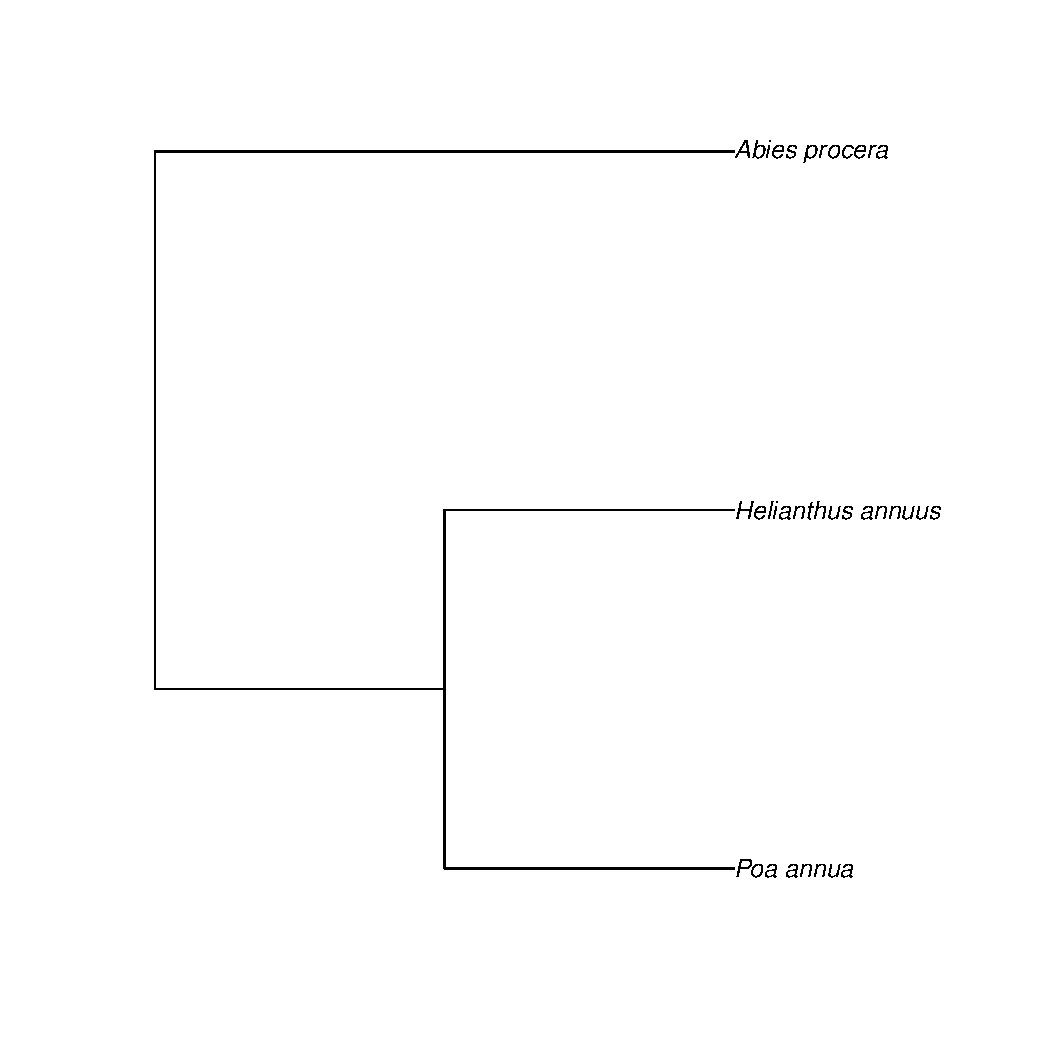
\includegraphics[width=4in,height=4in]{figure/phylomaticphylogeny} 

}

thing \textbf{shit} butt 


\end{knitrout}


Behind the scenes the function \emph{phylomatic\_tree} retrieves a Taxonomic Serial Number (TSN) from ITIS for each species name, then a string is created for each species like this \emph{}. These strings are submitted to the Phylomatic API, and if no errors occur, a phylogeny in newick format is returned. The \emph{phylomatic\_tree} also cleans up the newick string and converts to a ape \emph{phylo} object. The output from \emph{phylomatic\_tree} is a \emph{phylo} object, which can be used for plotting, phylogenetic analyses, etc. 

\subsection{What taxa are in children of my taxon of interest?}

If you aren't a taxonomic specialist on a particular taxon you likely don't know what children taxa are within a family, or within a genus. You can of course go to a website like Wikispecies (\url{http://species.wikimedia.org/wiki/Main_Page}) or Encyclopedia of Life (\url{http://eol.org/}). taxize provides an easy way for you to search for downstream taxa, both for the Catalogue of Life (CoL; \url{http://www.catalogueoflife.org/}) and the Integrated Taxonomic Information Database (\url{http://www.itis.gov/}). Here is a short example using the CoL in which we want to find all the species within the genus \emph{Apis} (honey bees).

\begin{knitrout}
\definecolor{shadecolor}{rgb}{0.969, 0.969, 0.969}\color{fgcolor}\begin{kframe}
\begin{alltt}
\hlfunctioncall{col_downstream}(name = \hlstring{"Apis"}, downto = \hlstring{"Species"})[[1]]
\end{alltt}
\begin{verbatim}
  childtaxa_id     childtaxa_name childtaxa_rank
1      6971712 Apis andreniformis        Species
2      6971713        Apis cerana        Species
3      6971714       Apis dorsata        Species
4      6971715        Apis florea        Species
5      6971716 Apis koschevnikovi        Species
6      6845885     Apis mellifera        Species
7      6971717   Apis nigrocincta        Species
\end{verbatim}
\end{kframe}
\end{knitrout}


\subsection{IUCN Status}

There are a number of things we can do once we have the correct taxonomic names. One thing we can do is ask about the conservation status of a species. We have provided a set of functions, \emph{iucn\_summary} and \emph{iucn\_status}, to search for species names, and extract the status information, respectively. Here, we search for the Panther and Lynx.  

\begin{knitrout}
\definecolor{shadecolor}{rgb}{0.969, 0.969, 0.969}\color{fgcolor}\begin{kframe}
\begin{alltt}
ia <- \hlfunctioncall{iucn_summary}(\hlfunctioncall{c}(\hlstring{"Panthera uncia"}, \hlstring{"Lynx lynx"}))
\hlfunctioncall{iucn_status}(ia)
\end{alltt}
\begin{verbatim}
Panthera uncia      Lynx lynx 
          "EN"           "LC" 
\end{verbatim}
\end{kframe}
\end{knitrout}


It turns out that the Panther is endangered (EN) and the Lynx is of least concern (LN). 

\section{Conclusion}

some text here

\section{Funding}

SAC is supported by CANPOLIN of Canada.

\section{Acknowledgements}

The taxize package is part of the rOpenSci project \url{http://ropensci.org/}.

\section{Appendices}

\begin{itemize}
    \item{Appendix A.} A complete reproducible workflow, from a species list to a phylogeny. 
\end{itemize}

\bibliography{refs}

\end{document}
